\documentclass[12pt]{article}
%encoding
%--------------------------------------
\usepackage[utf8]{inputenc}
\usepackage[T1]{fontenc}
\usepackage{listings}
\usepackage{minted}
\usepackage{mathtools}
\usepackage{graphicx}
\usepackage{placeins}  

\graphicspath{ {./img/} }
\def\code#1{\texttt{#1}}

%--------------------------------------

%German-specific commands
%--------------------------------------
\usepackage[ngerman]{babel}
%--------------------------------------

%Hyphenation rules
%--------------------------------------
\usepackage{hyphenat}
\hyphenation{Mathe-matik wieder-gewinnen}
\usepackage{lipsum}
%--------------------------------------
\begin{document}
\pagenumbering{gobble}
\clearpage
\thispagestyle{empty}
\author{Rafael Schreiber (5BHIF/KatNr. 20)}
\date{April 2021}
\title{POPpy \\ Ein minimalistischer POP3 Client \\ Aufgabe Nr. 29}
\maketitle
\begin{figure}[htbp]
    \centering
    
\includegraphics[scale=0.2]{poppy_logo}
    \label{fig:situation1}
\end{figure}
\FloatBarrier
\clearpage
\pagenumbering{arabic}
\tableofcontents
\newpage

\section{Einleitung}
\subsection{Aufgabenstellung}
Laut der Angabe soll ein einfacher POP3 Client programmiert werden, mit welchem
man E-Mails abrufen, herunterladen und löschen kann. Zudem sollte mithilfe von
GnuTLS \cite{gnutls} auch StartTLS unterstützt werden.
\newline
Eine weitere Anforderung ist, dass die Netzwerkbibliothek Asio \cite{asio} 
verwendet werden soll. Asio eine Bibliothek für eine moderne Netzwerk und 
low-level I/O Programierung mit einem konsitenten asynchronen Modell.

\subsection{Probleme}
\subsubsection{GnuTLS mit Asio}
Ein großes Problem bei der Programmierung mit Asio war, dass GnuTLS 
standardmäßig nicht die Asio Socket Objekte unterstützt. GnuTLS benötigt
nämlich den nativen Socket Deskriptor, auf welchem man bei Asio keinen Zugriff
hat.
\begin{minted}{c++}
    gnutls_transport_set_int(_sess, _socket_descriptor);
\end{minted}
Es gibt zwar GnuTLS Wrapper für Asio, diese sind aber nur kleine Projekte von 
einzelnen Entwicklern auf GitHub und außerdem sollten so wenige Bibliotheken 
wie möglich verwendet werden. Deshalb wurde auf Asio verzichtet und stattdessen 
die native POSIX Socket Bibliothek verwendet. GnuTLS funktioniert einfach damit
am besten.

\subsubsection{StartTLS}
StartTLS ist ein Verfahren zum herstellen einer gesicherten 
Netzwerkverbindung mittles TLS. Der unterschied zu implizitem TLS besteht
darin, dass der erste Verbindungsaufbau unverschlüsselt erfolgt. Das bietet die
Möglichkeit für einen möglichen Man-in-the-Middle-Angriff. 
\newline
\newline
Seit 2018 wird davon
abgeraten StartTLS für das Abrufen für E-Mails zu verwenden \cite{rfc8460}.
Auch weil StartTLS für POP3, sowohl als auch für IMAP, keinen Vorteil gegenüber 
implizitem TLS bietet und weil es praktisch keine POP3-Server mehr gibt, welche
auf StartTLS setzen, wurde auf dessen implementierung verzichtet und 
stattdessen auf "`herkömmliches"' TLS getzt. Zum Glück bietet GnuTLS auch eine 
Unterstützung für implizites TLS.

\section{Implementierung}
Zu aller erst wurden sämtliche Codierungsrichtlinien von Professor Dr. Günter 
Kolousek eingehalten. Für die Benennung von Variablen und Funktionen wurde
"`\code{sneak\_case}"' verwendet, ausgenommen die gRPC Implementierungen, weil
die vom gRPC-Compiler generierte C++ Bibliothek "`\code{PascalCase}"' nutzt.

\subsection{Architektur}
POPpy besteht aus einer klassischen Client-Server Architektur, mit dem 
Unterschied, dass Frontend und Backend via gRPC \cite{grpc} kommunizieren und 
nicht wie bei Web-Apps üblich mit einer REST-Schnittstelle. Das Backend ist in 
C++ programmiert und bietet deswegen auch eine hohe Geschwindigkeit. 
\newline
\newline
Das Frontend hingegen wurde in JavaScript programmiert, welches über eine HTML
Datei eingebunden wird. Dieses HTML File ist lokal gespeichert und wird beim 
starten von POPpy automatisch, wenn möglich, mit dem Standardprogramm für 
HTML Dateien, überlicherweise ein Webbrowser, vom Backend geöffnet.

\subsubsection{gRPC \& protobuf}
gRPC ist ein von Google entwickeltes open-source Remote Procedure Call (RPC) 
Framework. Mit gRPC kann der Client direkt Methoden auf dem Server aufrufen, 
auch wenn sich dieser nicht auf der gleichen Maschine befindet wie der Client.
Die Kommunikation bei gRPC erfolgt über HTTP/2 welches i. Allg. zwar schneller 
und sicherer ist aber keine Abwärtskompatibilität zu HTTP/1.1 bietet.
\newline
\newline
Dabei ist protobuf \cite{protobuf}, ebenfalls von Google entwickelt, für die 
Strukturierung der Daten verantwortlich. Deshalb ist protobuf ein integraler 
bestandteil von gRPC. Protobuf serialisiert strukturierte Daten anders wie JSON 
nicht text-basiert, sonder binär. Das reduziert die Nachrichtengröße, senkt 
dadurch auch den Traffic und steigert somit die Geschwindigkeit.

\paragraph{Probleme mit gRPC im Web:}
Wegen HTTP/2 Limitierungen in Browsern war gRPC eine lange Zeit Web-Entwicklern 
vorenthalten. Google widmete sich diesem Problem und entwickelte gRPC-Web.
\cite{grpc-web}
\newline
Das Problem wurde gelöst indem gRPC-Web HTTP/1.1 anstelle von HTTP/2 nutzt. Das
Problem mit der Abwärtskompatibilität wird mit einem Proxyserver gelöst. Google
empfiehlt auf ihrer Website zu gRPC-Web den Envoy Proxy \cite{envoy}.

\begin{figure}[htbp]
    \centering
    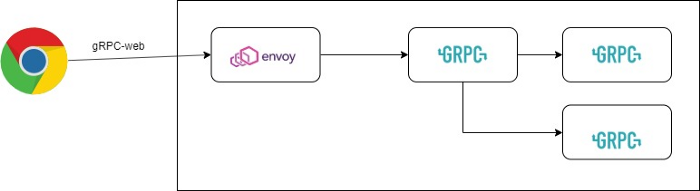
\includegraphics[scale=0.55]{grpc-web_communicaton}
    \caption{Kommunikation zwischen Browsern und gRPC Diensten \cite{abb1}}
    \label{fig:situation1}
\end{figure}
\FloatBarrier

\subsection{Aufbau}
\subsubsection{Frontend}
Das Frontend ist in JavaScript programmiert und wurde in einem npm Projekt
angelegt. Der Paketmanager npm eignet sich gut dafür, weil das Frontend mehrere
Bibliotheken benötigt darunter das wichtigste \code{grpc-web}. Dazu müssen
die vom protobuf- und gRPC-Compiler generierten Dateien im Frontend eingebunden
werden. Außerdem bietet webpack \cite{webpack} eine praktische Lösung alle 
Abhängigkeiten und Module in eine statische "`minified"' .js Datei 
zusammenzufassen welche dann einfach im HTML Dokument eingebunden wird.

\subsubsection{Backend}
Das Backend wurde in C++17 programmiert und bietet jeweils eine gRPC 
Schnittstelle für die Kommunikation mit dem Frontend und eine eigens
Programmierte API für den Datenaustausch mit dem POP3 Server Schnittstelle für 
die Kommunkation. Die Mailbox Klasse ist dafür zuständig, E-Mails während der
Laufzeit zu cachen, Verbindungen zu verwalten und eine einfache Repräsenatation
auf die E-Mails zu bieten.

\subsubsection{Envoy}
Envoy ist ein Proxy Server entwickelt von den Programmieren bei Lyft. Google 
selbst empfiehlt die Nutzung von Envoy bei gRPC-Web Applikationen. Envoy wird 
automatisch mit der richtigen Konfiguration vom Backend gestartet und 
verwaltet. Wenn Envoy abstürzt, dann schließt sich auch automatisch das 
Backend. Der Endanwender muss sich dabei um nichts kümmern.

\begin{figure}[htbp]
    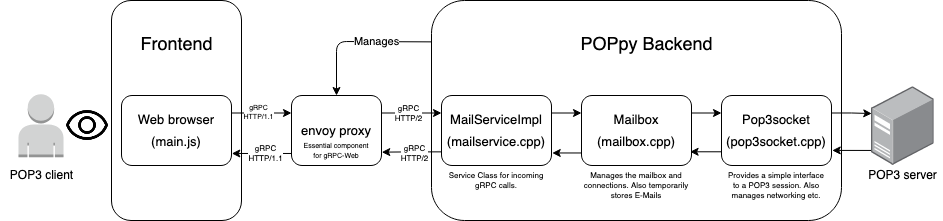
\includegraphics[scale=0.4]{poppy_app_diagram}
    \caption{Interne Programmstruktur von POPpy}
    \label{fig:situation2}
\end{figure}
\FloatBarrier

\subsection{Ablauf}
\subsubsection{Start}
POPpy wird über die Kommandozeile gestartet. Beim Start muss der Name eines
Bookmarks angegeben werden. Ein Bookmark gibt dabei Zugangsdaten zu einem POP3 
Server an. Bookmarks werden standardmäßig von der Datei 
\code{\textasciitilde /.config/poppy/poppy.conf} gelesen. Alternativ kann auch eine andere 
Datei angegeben werden. Diese TOML Datei ist folgendermaßen aufgabaut.
\begin{minted}{toml}
    # POPpy config file
    # This files contains bookmarks to your pop3 servers

    [beispielverbindung] # ERFORDERLICH
      host = "mail.domain.tld" # ERFORDERLICH
      port = 995               # Optional
      user = "user@domain.tld" # ERFORDERLICH
      pass = "changeit"        # NICHT EMPFOHLEN 
      ssl = true               # Optional 
\end{minted}
Wenn kein Passwort gespeichert wird, was auch Empfohlen ist, dann fragt POPpy
automatisch noch vor dem Start des Frontends nach dem Passwort. Wenn die Felder
\code{port} oder \code{ssl} nicht angegeben werden dann werden sie automatisch
auf 995 und true gesetzt. 
\newline
\newline
Beim Start werden zwei Threads gestartet. Diese werden mittels \code{async}
Aufruf als \code{future} in einem \code{vector<future<int>*>} gespeichert.
Diese Futures liefern als Integer einen Statuscode zurück. Diese Statuscodes
sind in der Datei \code{include/globals.h} gespeichert.
\newline
Der erste Thread startet und verwaltet den Envoy Proxy. Zum Starten wird die
Bibliothek \code{cpp-subprocess} verwendet. Die Funktion hinter diesem Thread 
sieht folgendermaßen aus:
\begin{minted}{c++}
int start_envoy_proxy() {
    auto envoy_process = Popen({"envoy", "-c", prefix + "/share/poppy/"
      "envoy_poppy_proxy.yaml", "--log-path", "/tmp/envoy_poppy.log.txt"}, 
      input{PIPE}, output{"/dev/null"});
    envoy_process_pid = envoy_process.pid();
    logger->debug("Envoy proxy started with pid: {}", envoy_process_pid);
    logger->debug("Check envoy log file after exit under "
      "/tmp/envoy_poppy.log.txt");
    logger->debug("You can also access the envoy admin panel under "
      "http://localhost:42963");
    size_t envoy_exit_status = envoy_process.wait();

    if (envoy_exit_status != SUCCESS) {
        logger->warn("Envoy proxy (PID: {}) exited with status code: {}",
          envoy_process_pid, envoy_exit_status);
        envoy_error = true;
    } else {
        logger->debug("Envoy proxy (PID: {}) exited with status code: {}",
          envoy_process_pid, envoy_exit_status);
    }
    return envoy_exit_status;
}
\end{minted}
Während der zweite Thread startet, wartet dieser davor ob Envoy richtig
gestartet hat. Falls das nicht der Fall sein sollte, dann verweigert dieser den
Start. Ein Teil der Funktion hinter dem zweiten Thread sieht so aus:
\begin{minted}{c++}
int start_grpc_server() {
    /* ... */
    int status = service->ConnectMailService(cred.hostname, cred.port, 
      cred.username, cred.password, cred.encrypted);
    if (status != SUCCESS) {
        logger->error("An error occurred while starting the gRPC service");
        free(service);
        return status;
    }
    
    grpc::ServerBuilder builder;
    builder.AddListeningPort(server_addr, grpc::InsecureServerCredentials());
    builder.RegisterService(service);
    server = builder.BuildAndStart();
    logger->info("gRPC server successfully started and is now "
      "listening on: {}", server_addr);
    thread check_shutdown_thread(check_shutdown);
    
    if (open_frontend() != SUCCESS) { 
        logger->warn("Failed to start frontend. Please open the html file "
          "manually located under: {}/share/poppy/index.html", prefix); 
    }

    server->Wait();
    check_shutdown_thread.join();
    service->ExitMailService();
    server->Shutdown();
    free(service);
    return SUCCESS;
}
\end{minted}
Die Variablen \code{cred} und \code{service} sind dabei globale Variablen.
Davon ist \code{service} ein Pointer zum gRPC Service und \code{cred} ein 
Objekt vom Typ \code{cred\textunderscore t}, welches vom Bookmark Parser mit 
den Zugangsdaten befüllt wird.
\newline
Die Methode \code{ConnectMailService} startet die Mailbox, welche dann im
Endeffekt mithilfe von Pop3socket die POP3 Sitzung startet. Wenn die Sitzung 
gestartet ist hört der gRPC Dienst nach eingehenden RPCs.

\subsubsection{Laufzeit}
Der gRPC Service nimmt eingehende Verbindungen und RPCs an und bearbeitet sie.
Die Daten bekommt der Dienst von dem Mailbox Objekt welches er beim Start
angelegt hat. Die RPC Handler Funktionen sehen so aus:
\begin{minted}{c++}
class MailServiceImpl final : public MailService::Service {
  private:
    Mailbox _pop3mailbox{};
    std::string _account;

  public:
    MailServiceImpl() {}
    int ConnectMailService(std::string hostname, uint16_t port, 
      std::string username, std::string password, bool encrypted);
    grpc::Status GetMailBoxInfo(grpc::ServerContext* context, 
      const Empty* request, MailBoxInfo* reply) override;
    grpc::Status GetMailPreviews(grpc::ServerContext* context, 
      const MailPreviewRequest* request, MailPreviewResponse* reply) override;
    grpc::Status UpdateMailbox(grpc::ServerContext* context, 
      const Empty* request, StatusResponse* reply) override;
    grpc::Status DeleteMail(grpc::ServerContext* context, 
      const SpecifiedMail* request, StatusResponse* reply) override;
    grpc::Status ResetMailbox(grpc::ServerContext* context, 
      const Empty* request, StatusResponse* reply) override;
    grpc::Status DownloadMail(grpc::ServerContext* context, 
      const SpecifiedMail* request, DownloadedMail* reply) override;
    grpc::Status ExitApplication(grpc::ServerContext* context, 
      const Empty* request, StatusResponse* reply) override;
    void ExitMailService();
    ~MailServiceImpl() {}

};
\end{minted}
Das ist die einzige Klasse, welche in "`\code{PascalCase}"' geschrieben ist.
\newline
Beim Start der Mailbox Klasse wird außerdem ein Thread gestartet,
welcher alle 10 Sekunden den POP3 Server "`anpingt"' um zu Kontrollieren ob die
Verbindung noch aufrecht ist und damit der Server die Verbindung nicht wegen
inaktivität abbricht. Diese dazugeörige Funktion zu diesem Ping Thread sieht so
aus:
\begin{minted}{c++}
void Mailbox::_ping_thread_function() {
    int noop_status;
    this_thread::sleep_for(10000ms);

    while (!shutdown_initiated) {
        if (_pop3sess.in_update_state()) {
            noop_status = _pop3sess.ping();
            if (noop_status != SUCCESS) break;
        }
        this_thread::sleep_for(10000ms);
    }

    if (!shutdown_initiated) {
        logger->error("Connection timeout. Server is not reachable. Initiating"
          " shutdown...");
        shutdown_initiated = noop_status;
    }
}
\end{minted}
Die Variable \code{shutdown\textunderscore initiated} ist dabei eine 
Hilfsvariable welche in­di­zie­rt, ob das Backend gestoppt wird unabhängig davon 
ob der Nutzer POPpy geschlossen hat oder irgendein Fehler aufgetreten ist.

\subsubsection{Shutdown}
Wie vorhin erwähnt wird beim Herunterfahren die Variable 
\code{shutdown\textunderscore initiated} gesetzt welche jedem Thread mitteilt, 
dass er sich beenden soll. So auch der Thread der Funktion 
\code{void check\textunderscore shutdown()} . Dieser Thread wird in der 
Funktion \code{int start\textunderscore grpc\textunderscore server()} gestartet
und beendet sich selbst sowie den gRPC Server wenn die 
\code{shutdown\textunderscore initiated} Variable gesetzt wurde. Die Funktion
zu diesem Thread ist sehr minimal und sieht so aus:
\newpage
\begin{minted}{c++}
void check_shutdown(){
    while (!shutdown_initiated) {
        this_thread::sleep_for(1000ms);
    }
    logger->info("gRPC server successfully shut down");
    server->Shutdown();
}
\end{minted}
Während sich der gRPC Server beendet, wird auch der Envoy Proxy mittels 
\code{SIGTERM} beendet. Wenn alle Dienste beendet sind terminiert das Programm.

\section{Verwendung}
\subsection{Abhängigkeiten}
Zuerst müssen folgende Programme installiert sein oder zumindest in 
\code{\$PATH} vorhanden sein. Meson überprüft vor dem kompilieren, ob diese 
vorhanden sind, wenn das nicht der Fall ist, dann wird bei einem Fehler der 
Link zum Download ausgegeben.
\begin{itemize}
    \item Einen C++ Compiler
    \item The Meson Build System \cite{meson}
    \item protobuf \cite{protobuf}
    \item gRPC mit protoc-gen-grpc-web \cite{protoc-gen-grpc-web}
    \item Envoy Proxy \cite{envoy}
    \item npm \cite{npm}
\end{itemize}
Daneben werden außerdem auch noch  Bibliotheken benötigt:
\begin{itemize}
    \item GnuTLS \cite{gnutls}
    \item GNU Mailutils \cite{mailutils}
\end{itemize}
\newpage
Dazu kommen noch ein paar Header-Only Bibliotheken, dessen Elternpfade in der 
Datei \code{meson\textunderscore options.txt} angegeben werden:
\begin{itemize}
    \item CLI11 \cite{cli11}
    \item cpp-subprocess \cite{cpp-subprocess}
    \item spdlog \cite{spdlog}
    \item toml++ \cite{toml}
\end{itemize}

\subsection{Komplilierung}
Zuerst wechselt man in den Ordner \code{build/}, dieser sollte zu beginn leer
sein. Danach kann Meson mit folgendem Befehl gestartet werden:
\begin{minted}{shell}
    $ meson --prefix $PWD/.. ..
    # Falls das Programm danach auch installiert werden soll, dann 
    # sollte bei --prefix der gewünschte Installationspfad angegeben 
    # werden. Zum Beispiel /usr/local
\end{minted}
Währenddessen überprüft Meson, ob auch alle Abhängigkeiten installiert sind.
Eine Ausnahme dabei ist GNU Mailutils. Außerdem werden auch alle protobuf und
gRPC Dateien generiert und das Frontend via npm kompiliert. Dieser Befehl
könnte deshalb ein wenig länger dauern. \newline
Zum kompilieren danach folgenden Befehl ausführen
\begin{minted}{shell}
    $ ninja
\end{minted}
Falls gewünscht kann das Programm danach auch installiert werden:
\begin{minted}{shell}
    $ meson install
\end{minted}
Die Kompilierung wurde auf folgenden Plattformen getestet:
\begin{itemize}
    \item macOS Big Sur (Apple clang version 12.0.0)
    \item Ubuntu 20.04 LTS (gcc version 9.3.0)
\end{itemize}
Beide Plattformen basieren auf einen Prozessor mit x86 Befehlssatz.

\subsection{Benutzung}
Vor dem ersten Start muss die Datei 
\code{\textasciitilde /.config/poppy/poppy.conf} bearbeitet werden. Dort 
einfach ein Bookmark mit den Anmeldedaten definieren und speichern. 
\newline
\newline
\textbf{Achtung! Falls POPpy nicht installiert wurde, muss die Datei 
manuell erstellt werden. Eine Beispielkonfiguration ist unter 
\code{poppy\textunderscore sample.conf}.}

\subsubsection{Kommandozeilenparameter}
\paragraph{bookmark TEXT REQUIRED:}
Gibt den Namen des Bookmarks an zu welchem eine POP3 Sitzung hergestellt werden 
soll.

\paragraph{-c,--config TEXT:FILE OPTIONAL:}
Falls nicht die Standard Konfigurationsdatei unter 
\code{poppy\textunderscore sample.conf} verwendet werden soll, kann mit diesem
Parameter eine alternative Datei angegeben werden.

\paragraph{-d,--debug:}
Wenn dieser Flag gesetzt ist, wird POPpy im Debug Modus gestartet. Dieser Modus
bietet mehr Transparenz über die Abläufe im Programm und ist hilfreich bei
Fehlern.

\begin{thebibliography}{25}
\bibitem{gnutls} 
The GnuTLS Transport Layer Security Library
\\\textit{https://www.gnutls.org}

\bibitem{asio} 
Asio C++ Library
\\\textit{https://think-async.com/Asio}

\bibitem{rfc8460} 
SMTP TLS Reporting
\\\textit{https://tools.ietf.org/html/rfc8460}

\bibitem{grpc} 
gRPC: A high performance, open source universal RPC framework
\\\textit{https://grpc.io/docs/what-is-grpc/introduction}

\bibitem{protobuf} 
Protocol Buffers | Google Developers
\\\textit{https://developers.google.com/protocol-buffers}

\bibitem{grpc-web} 
A basic tutorial introduction to gRPC-web.
\\\textit{https://grpc.io/docs/platforms/web/basics/}

\bibitem{envoy} 
Envoy Proxy - Home
\\\textit{https://www.envoyproxy.io/}

\bibitem{npm}
npm (Node Package Manager)
\\\textit{https://www.npmjs.com}

\bibitem{abb1}
Ditching REST with gRPC-web and Envoy
\\\textit{https://medium.com/swlh/ditching-rest-with-grpc-web-and-envoy-bfaa89a39b32}

\bibitem{webpack}
webpack
\\\textit{https://webpack.js.org}

\bibitem{protoc-gen-grpc-web}
protoc-gen-grpc-web
\\\textit{https://github.com/grpc/grpc-web/releases}

\bibitem{meson} 
The Meson Build System: Project Website
\\\texttt{https://mesonbuild.com}

\bibitem{mailutils} 
GNU Mailutils: General-Purpose Mail Package
\\\texttt{https://mailutils.org}

\bibitem{cli11} 
GitHub: CLIUtils/CLI11 command line parser
\\\texttt{https://github.com/CLIUtils/CLI11}

\bibitem{cpp-subprocess} 
GitHub:  arun11299/cpp-subprocess Subprocessing with modern C++ 
\\\texttt{https://github.com/arun11299/cpp-subprocess}

\bibitem{spdlog} 
GitHub:  gabime/spdlog Fast C++ logging library. 
\\\texttt{https://github.com/gabime/spdlog}

\bibitem{toml} 
GitHub:  marzer/tomlplusplus Header-only TOML config file parser and serializer
\\\texttt{https://github.com/marzer/tomlplusplus}

\end{thebibliography}

\end{document}